\section{Introduction}
\label{sec:introduction}

Vision--language--action policies map natural-language goals and images directly to robot motion \cite{kim2024openvla,black2024pi0,shukor2025smolvla}. Their language input is semantic and hierarchical---``put the soup and tomato in the basket'' implies multiple object-conditioned stages---but their output interface is typically a uniform array of future joint or end-effector waypoints. This mismatch becomes consequential over long horizons. A fixed chunk has neither an explicit semantic boundary nor an independent physical clock, so language must select a behavior, encode its detailed geometry, and implicitly determine how long it should run through the same dense output array.

We ask whether the action interface itself can make a VLA easier to address with language. Our answer is a \emph{language-addressable spline action program} (\method; Fig.~\ref{fig:overview}). Each policy query predicts a compact cubic B-spline trajectory, a gripper curve, and the duration to the next manipulation event. A long instruction is represented as executable clauses; each clause conditions the same policy until a clock advances the program. Normalized spline phase $u\in[0,1]$ represents trajectory shape, while duration $T$ supplies physical time. This separation also makes rate and speed changes decode-time operations on a fixed learned geometry.

The central question is not whether language decomposition helps in general, but whether the action representation changes how much it helps. We therefore conduct a matched $2\!\times\!2$ experiment: stock 50-waypoint SmolVLA versus the spline-duration head, crossed with a whole-task caption versus executable clauses. All four conditions use exactly the same 71 demonstrations and 19,378 physical frames; only the action targets and text view change. Across three training seeds on two LIBERO-Long tasks, clauses improve waypoint success by 34.3 percentage points (pp) and spline success by 43.7~pp. The difference-in-differences is +9.33~pp and is positive for every seed (hierarchical 95\% CI, 0.67--18.0). Static compound-prompt controls regress, showing that the gain comes from executing the language units rather than merely fine-tuning on longer text.

Behavioral interventions and cross-domain tests support the mechanism. Reversing the clause order changes the requested first completed object in 10/50 paired LIBERO states for each head, with no changes in the opposite direction. Official semantic phases raise two-task RoboCasa365 success from 4/100 to 16/100 on one seed and from 3/40 to 9/40 on an independent seed. Finally, the same geometry--time factorization yields a second, complementary capability: retiming a learned spline on CALVIN improves average five-instruction chain length by 0.379 while increasing realized speed by 1.42$\times$, and resampling repairs a LIBERO control-rate failure from 38\% to 68\% and from 34\% to 72\% under two protocols.

\begin{figure*}[t]
    \centering
    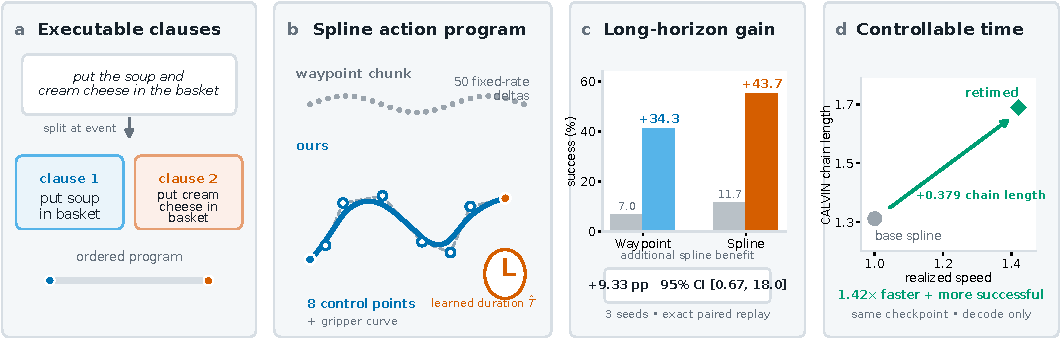
\includegraphics[width=\textwidth]{figures/overview.pdf}
    \caption{\textbf{Language-addressable spline action programs.} A long-horizon instruction is scheduled as executable clauses. For each clause, the VLA predicts eight control points for a continuous path, a gripper curve, and event duration $T$, rather than a dense fixed-rate waypoint array. The matched experiment isolates an additional +9.33~pp clause benefit for the spline head; the same shape--time factorization supports successful decode-time retiming on CALVIN.}
    \label{fig:overview}
\end{figure*}

Our contributions are:
\begin{itemize}
    \item an event-aligned spline VLA head that jointly predicts compact path geometry, gripper state, and physical duration without modifying the vision--language backbone;
    \item a controlled, three-seed executable-language study showing that clauses improve both action heads but improve the spline head significantly more, together with order interventions and RoboCasa365 replication; and
    \item a unified time-control study showing that the same learned head supports event scheduling, language-conditioned pace, temporal rescaling, and control-rate adaptation at decode time.
\end{itemize}
